\documentclass{article}[12pt]
\usepackage{color}
\usepackage[normalem]{ulem}
\usepackage{times}
\usepackage{fullpage}
\usepackage{amsmath}
\usepackage{amssymb}
\usepackage{listings}
\usepackage{tikz}
\def \R {\mathbb R}
\def \imp {\Longrightarrow}
\def \eps {\varepsilon}
\def \Inf {{\sf Inf}}
\newenvironment{proof}{{\bf Proof.  }}{\hfill$\Box$}
\newtheorem{theorem}{Theorem}[section]
\newtheorem{definition}{Definition}[section]
\newtheorem{corollary}{Corollary}[section]
\newtheorem{lemma}{Lemma}[section]
\newtheorem{claim}{Claim}[section]
\setlength {\parskip}{2pt}
\setlength{\parindent}{0pt}

\newcommand{\headings}[4]{\noindent {\bf Assignment 14 CME241} \hfill {{\bf Author:} Nicolas Sanchez} \\
{} \hfill {{\bf Due Date:} #2} \\

\rule[0.1in]{\textwidth}{0.025in}
}

\newcommand{\klnote}[1]{{\color{red} #1}}
\newcommand{\klsout}[1]{{\color{red} \sout{#1}}}

\begin{document}

\headings{\#1}{Tuesday, October 8, 10:30am}\section{} 



\section{LSTD and LSPI Algorithm Implementations}
We implement the two algorithms generically:

\begin{lstlisting}
class LSTD(FunctionApprox[X]):
    A_matrix:np.ndarray
    b_vector:np.ndarray
    w:np.ndarray
    feat_func: Callable[[X],np.ndarray]

    def __init__(
        self,
        num_feats: int,
        feat_func: Callable[[X],np.ndarray],
    ):
        self.feat_func = feat_func
        self.A_matrix: np.ndarray = np.zeros((num_feats,num_feats))
        self.b_vector: np.ndarray = np.zeros(num_feats)
        self.w: np.ndarray = np.zeros(num_feats)
        super().__init__()

    ########### MUST MEET FUNCTIONAPPROX SPEC ###############
    def update(
        self,
        xy_vals_seq: Iterable[Tuple[X, float]]
    ) -> FunctionApprox[X]:
        return self

    def solve(
        self,
        xy_vals_seq: Iterable[Tuple[X, float]],
        error_tolerance: Optional[float] = None
    ) -> FunctionApprox[X]:
        return self

    def representational_gradient(self, x_value: X) -> FunctionApprox[X]:
        return self

    def evaluate(self, x_values_seq: Iterable[X]) -> np.ndarray:
        return np.array([np.dot(self.weights, self.feat_func(x)) for x in x_values_seq])

    def within(self, other: FunctionApprox[X], tolerance: float) -> bool:
        return False

    ########### ADDITIONAL FUNCTIONS #######################
    def train_up(self, s1: X, rew: float, s2: X, gamma:float, term: bool) -> None:
        s1_feat = self.feat_func(s1)
        s2_feat = self.feat_func(s2)
        self.A_matrix += s1_feat.T.dot(s1_feat - gamma*s2_feat*(1-float(int(term))))
        self.b_vector+= rew*s1_feat*gamma

    def update_weights(self, normalization = 1.0, reg_val = 0.001) -> None:
        self.A_matrix *=normalization 
        self.b_vector *=normalization
        self.A_matrix += reg_val*np.eye(self.b_vector.shape[0])
        self.w = np.linalg.inv(self.A_matrix).dot(self.b_vector)

    def reset_count(self) -> None:
        self.A_matrix = np.zeros((num_feats,num_feats))
        self.b_vector =np.zeros(num_feats)

    def evaluate_vf(self, s: X) -> float:
        s_feat = feat_func(s)
        return np.dot(self.w, s_feat)


def LSPI(
        replay_memory: Distribution[TransitionStep[S, A]],
        mdp: MarkovDecisionProcess[S,A],
        feat_funct: Callable[Tuple[S,A],np.ndarray],
        dim_feat: int,
        batch_size: int,
        eps: float,
        gamma: float
) -> Iterable[FunctionApprox]:
    lstqd_approx = LSTD(num_feats =dim_feat, feat_func = feat_func, gamma = gamma) 
    while(True):
        curr_policy = markov_decision_process.policy_from_q(lstqd_approx, mdp, eps)
        for tr_step in replay_memory.sample_n(batch_size):
            next_action = curr_policy.act(tr_step.next_state)
            lstsq.train_up((tr.state,tr.action),tr.reward,(tr.next_state, next_action),\
                gamma, mdp.is_terminal(next_state))
        lstsq.update_weights()
        yield lstqd_approx
\end{lstlisting}

We then attempt to implement our own personalized version of the LSPI for the American Options Pricing but unfortunately do not attain results similar to the ones attained by the code in the repo (despite using similar steps). Here is our implementation excluding definitions of constant (can be found in LSPI\_American\_Option.py:

\begin{lstlisting}
 def payoff_func(_: float, s: float) -> float:
        return max(strike - s, 0.)


    #### create LSPI object
    num_feats = 7
    num_laguerre: int = 3
    ident: np.ndarray = np.eye(num_laguerre)
    feat_func = lambda ts : np.array([\
            1.,\
            np.exp(-ts[1] / (2 * strike)) *\
                  lagval(ts[1] / strike, ident[0]),\
            np.exp(-ts[1] / (2 * strike)) *\
                  lagval(ts[1] / strike, ident[1]),\
            np.exp(-ts[1] / (2 * strike)) *
                  lagval(ts[1] / strike, ident[2]),\
            np.cos(-ts[0] * np.pi / (2 * expiry_val)),
            np.log(expiry_val - ts[0]) if ts[0] != expiry_val else 0.,
            (ts[0] / expiry_val) ** 2 ])
    lstd_approx = LSTD(num_feats, feat_func)


    ### run simulations and updates
    ret: List[TrainingDataType] = []
    spot: float = spot_price_val
    vol2: float = vol_val * vol_val

    mean2: float = spot * spot
    var: float = mean2 * spot_price_frac_val * spot_price_frac_val
    log_mean: float = np.log(mean2 / np.sqrt(var + mean2))
    log_stdev: float = np.sqrt(np.log(var / mean2 + 1))
    gamma: float = np.exp(-rate_val * dt)
    for train_iter in range(lspi_training_iters):
        print("Training Iteration number ", train_iter )
        for i in range(num_training_paths):
            price: float = np.random.lognormal(log_mean, log_stdev)
            for step in range(num_steps_val):
                m: float = np.log(price) + (rate_val - vol2 / 2) * dt
                v: float = vol2 * dt
                next_price: float = np.exp(np.random.normal(m, np.sqrt(v)))
                state = (step*dt,price)
                next_state = ((step+1)*dt,next_price)
                ex: bool = lstd_approx.evaluate_vf(next_state) > payoff_func(*next_state)
                term: bool = step+1 == num_steps_val
                keep:bool = not( ex or term)
                lstd_approx.train_up(
                    state,\
                    0.0 if keep else payoff_func(*next_state),\
                    next_state,\
                    gamma,\
                    not keep)
                price = next_price

        lstd_approx.update_weights(normalization = 1./float(num_training_paths*num_steps_val))
        print(lstd_approx.w)
        lstd_approx.reset_count()
\end{lstlisting}


We find more encouraging results when implementing the DQL. After the training we compare the value of the approximation with the payoff to determine the option execution boundary at time 0.5 and we find a price of 79 (see image below) which is close to the result found in class - however more testing would be needed. Our implementation similar to LSPI is also below.

\begin{figure}[h]
  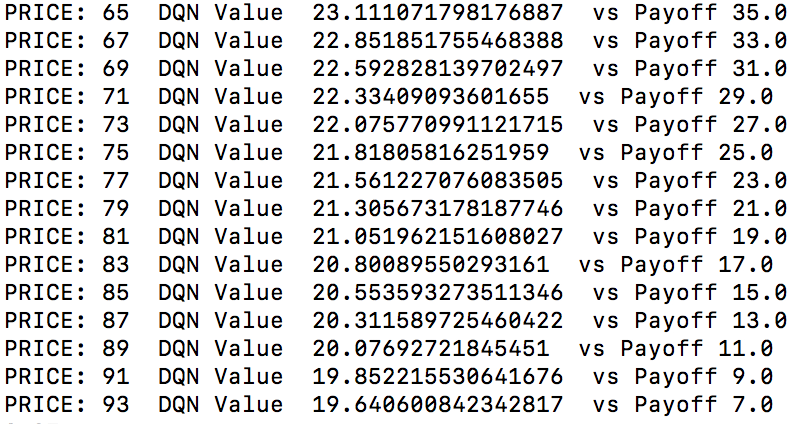
\includegraphics[width=\linewidth]{output_dql.png}
  \caption{Output from DQL after training for time 0.5}
  \label{fig:optPol1}
\end{figure}


\begin{lstlisting}
   feat_func_dql=[
        lambda t_s: 1.,
        lambda t_s: t_s[0] / expiry_val,
        lambda t_s: t_s[1] / strike,
        lambda t_s: t_s[0] * t_s[1] / (expiry_val * strike)
    ]

    dnn_spec: DNNSpec = DNNSpec(
        neurons=[1],
        bias=True,
        hidden_activation=lambda x: np.log(1 + np.exp(-x)),
        hidden_activation_deriv=lambda y: np.exp(-y) - 1,
        output_activation=lambda x: x,
        output_activation_deriv=lambda y: np.ones_like(y)
    )


    adam = AdamGradient(
            learning_rate=0.1,
            decay1=0.9,
            decay2=0.999
        )
    dnn_appr = DNNApprox.create(
            feature_functions=feat_func_dql,
            dnn_spec=dnn_spec,
            adam_gradient=adam,
            regularization_coeff=1e-6
        )

    dql_count = 0 
    while True:
        for i in range(num_training_paths):
            price: float = np.random.lognormal(log_mean, log_stdev)
            for step in range(num_steps_val):
                m: float = np.log(price) + (rate_val - vol2 / 2) * dt
                v: float = vol2 * dt
                next_price: float = np.exp(np.random.normal(m, np.sqrt(v)))
                state = (step*dt,price)
                next_state = ((step+1)*dt,next_price)
                if step+1 == num_steps_val:
                    rew = payoff_func(*next_state)
                else:
                    rew = max(dnn_appr(next_state), payoff_func(*next_state))
                dnn_appr = dnn_appr.update([(state, rew*gamma)])
                price = next_price
                dql_count += 1
            t = 0.5
            if dql_count % 10000 == 0:
                print(float(dql_count/dql_training_iters))
                for price in range(65,95,2):
                    print("PRICE:", price, " DQN Value ",dnn_appr((0.5,price)), " vs Payoff", payoff_func(0.5, price))
            if dql_count > dql_training_iters:
                    break
        if dql_count > dql_training_iters:
            break

\end{lstlisting}
\end{document}
